\label{backscatter section}
%----------------------------------------------------------------------------
Consider an optical setup where a laser beam line is merged with receiver beam line. The merge could be facilitated through the use of a dichroic beam splitter: reflecting the wavelength associated with the laser while transmitting the broad spectrum associated with the fluorescence radiation. By allowing some of the laser focusing optics to double as the receiver optics gives rise to unique geometries where the receiver and laser source are localized and their beam lines are extended to some remote target region (a LIDAR application). See Figure \ref{backscatter_figure} for a beam line diagram.
%----------------------------------------------------------------------------
%----------------------------------------------------------------------------
%bb defines the bounding box for the pdf
%viewport defines the area of the pdf used
%in sidewaysfigure the last entry in bb moves the caption toward/away the pic
%in sidewaysfigure the second entry in bb moves the pic toward/away the caption
%----------------------------------------------------------------------------
\begin{figure}
\scalebox{0.6}[0.6]{
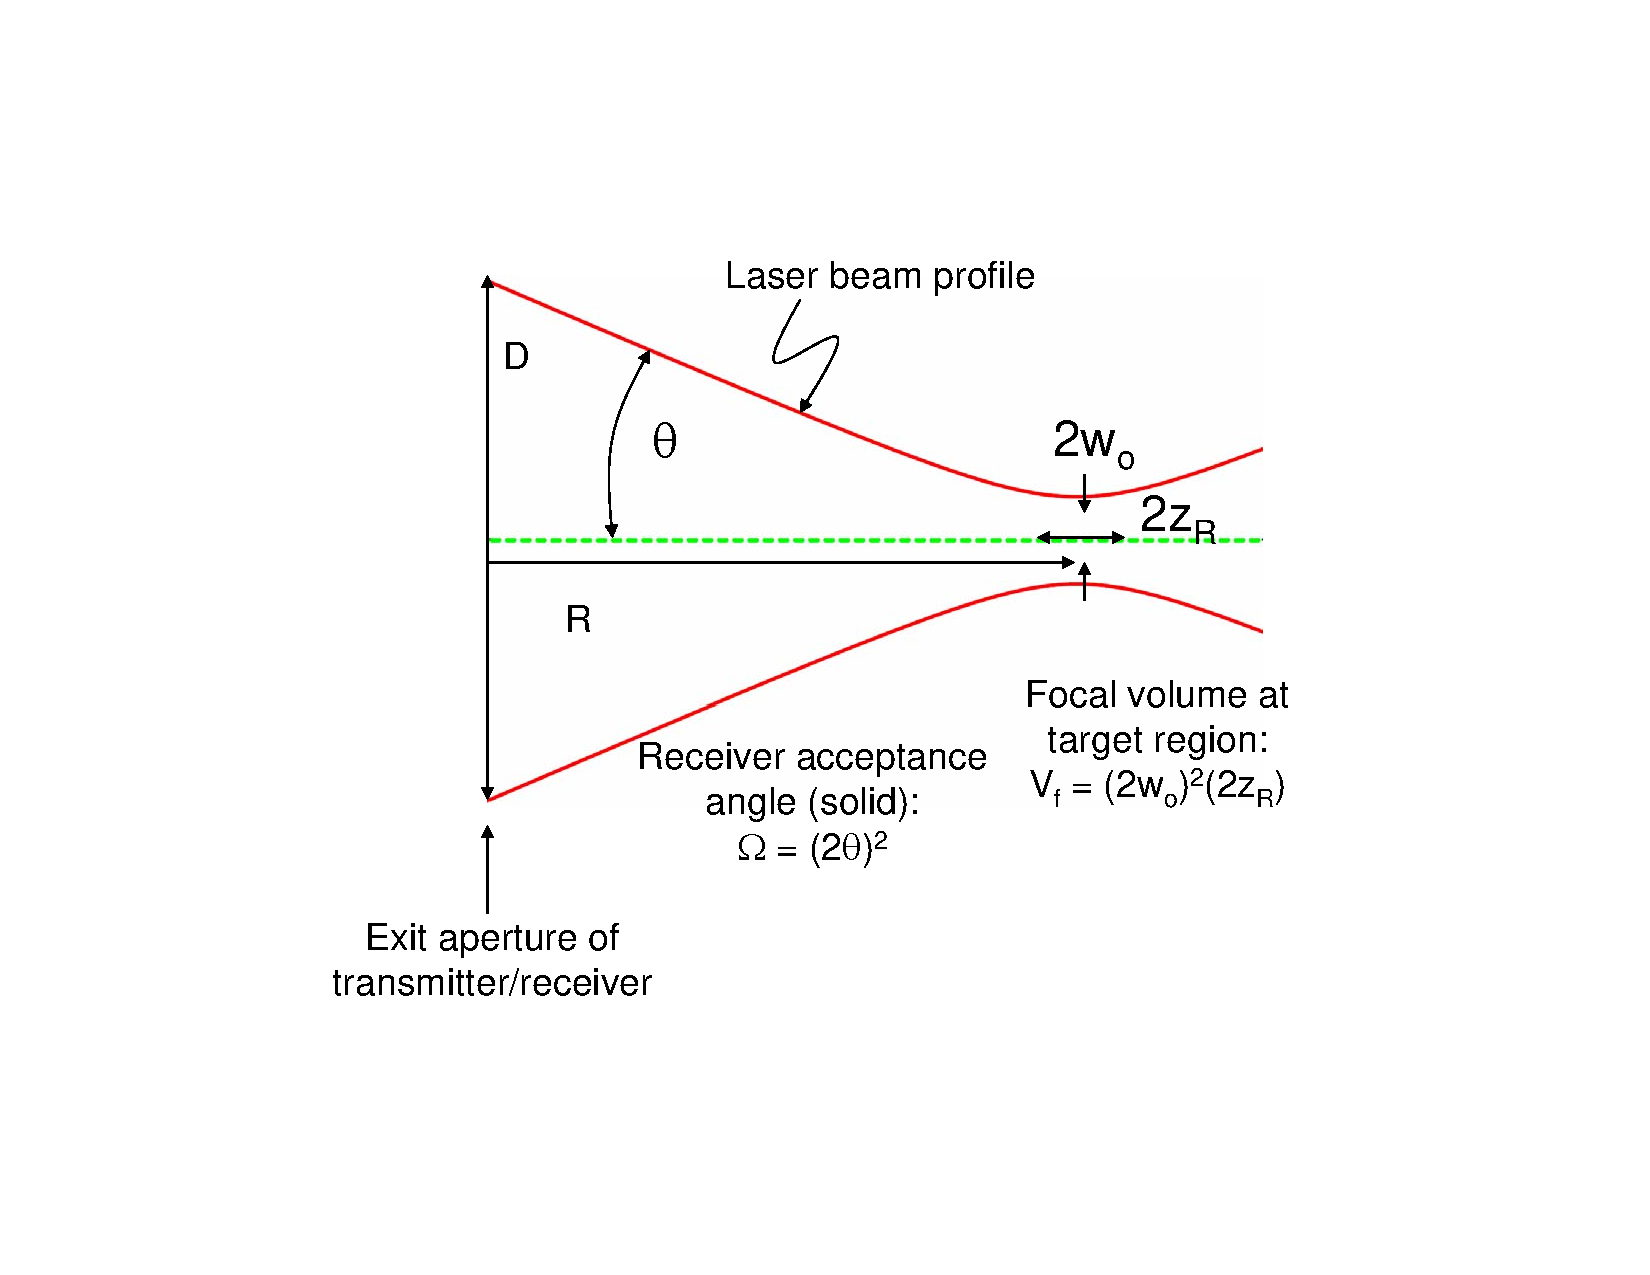
\includegraphics[bb=35 125 489 480]
{backscatter_figure/backscatter_figure.pdf}
}
\caption[Backscatter geometry]{Backscatter geometry. After leaving the exit aperture of diameter D, a laser beam is brought to a focus a distance R from the aperture. The dimensions of the focal volume and the far-field divergence ($\theta$) depend only on D, R, and the laser wavelength $\lambda$.}
\label{backscatter_figure}
\end{figure}
%----------------------------------------------------------------------------

%----------------------------------------------------------------------------

The probability of photon detection is proportional to
%----------------------------------------------------------------------------
\begin{equation}
ABCD
\int\int
\rho(\vec{r})
P(\vec{r},t)
\Phi(\vec{r},\hat{c})
d\vec{r}
d\Omega
\label{total_prob}
\end{equation}
%----------------------------------------------------------------------------
where $A$ is the fraction of target molecules which couple to the laser radiation, $B$ represents atmospheric attenuation effects like Mie scattering, absorption, etc., $C$ represents the fraction of excited molecules that decay optically within the bandwidth of the detector, $D$ represents the fraction of optically decaying molecules which emit a photon before collisional effects force non-optical decay (see discussion at the end of Section \ref{side}), $\rho(\vec{r})$ is the density distribution of the target molecules, $P(\vec{r},t)$ is the molecular inversion probability (this is a function of the fluence at position $\vec{r}$ and at time $t$), $\Phi(\vec{r},\hat{c})$ is the phase space factor (a function of position as well as the direction of travel of the emitted photon $\hat{c}$). In the following analysis some approximations are made to estimate this integral. First we ignore $A$, $B$, $C$, and $D$, thus we simply calculate the photon capture probability assuming all molecules optically decay isotropically. The density is assumed uniform, $\Phi$ is simply taken to limit the integration volume to the focal volume and introduce a factor equal to the solid angle fraction available to the detector from the target region, and $P$ is assumed to be equal to unity.
%----------------------------------------------------------------------------
%----------------------------------------------------------------------------
%bb defines the bounding box for the pdf
%viewport defines the area of the pdf used
%in sidewaysfigure the last entry in bb moves the caption toward/away the pic
%in sidewaysfigure the second entry in bb moves the pic toward/away the caption
%----------------------------------------------------------------------------
\begin{figure}
\scalebox{0.8}[0.8]{
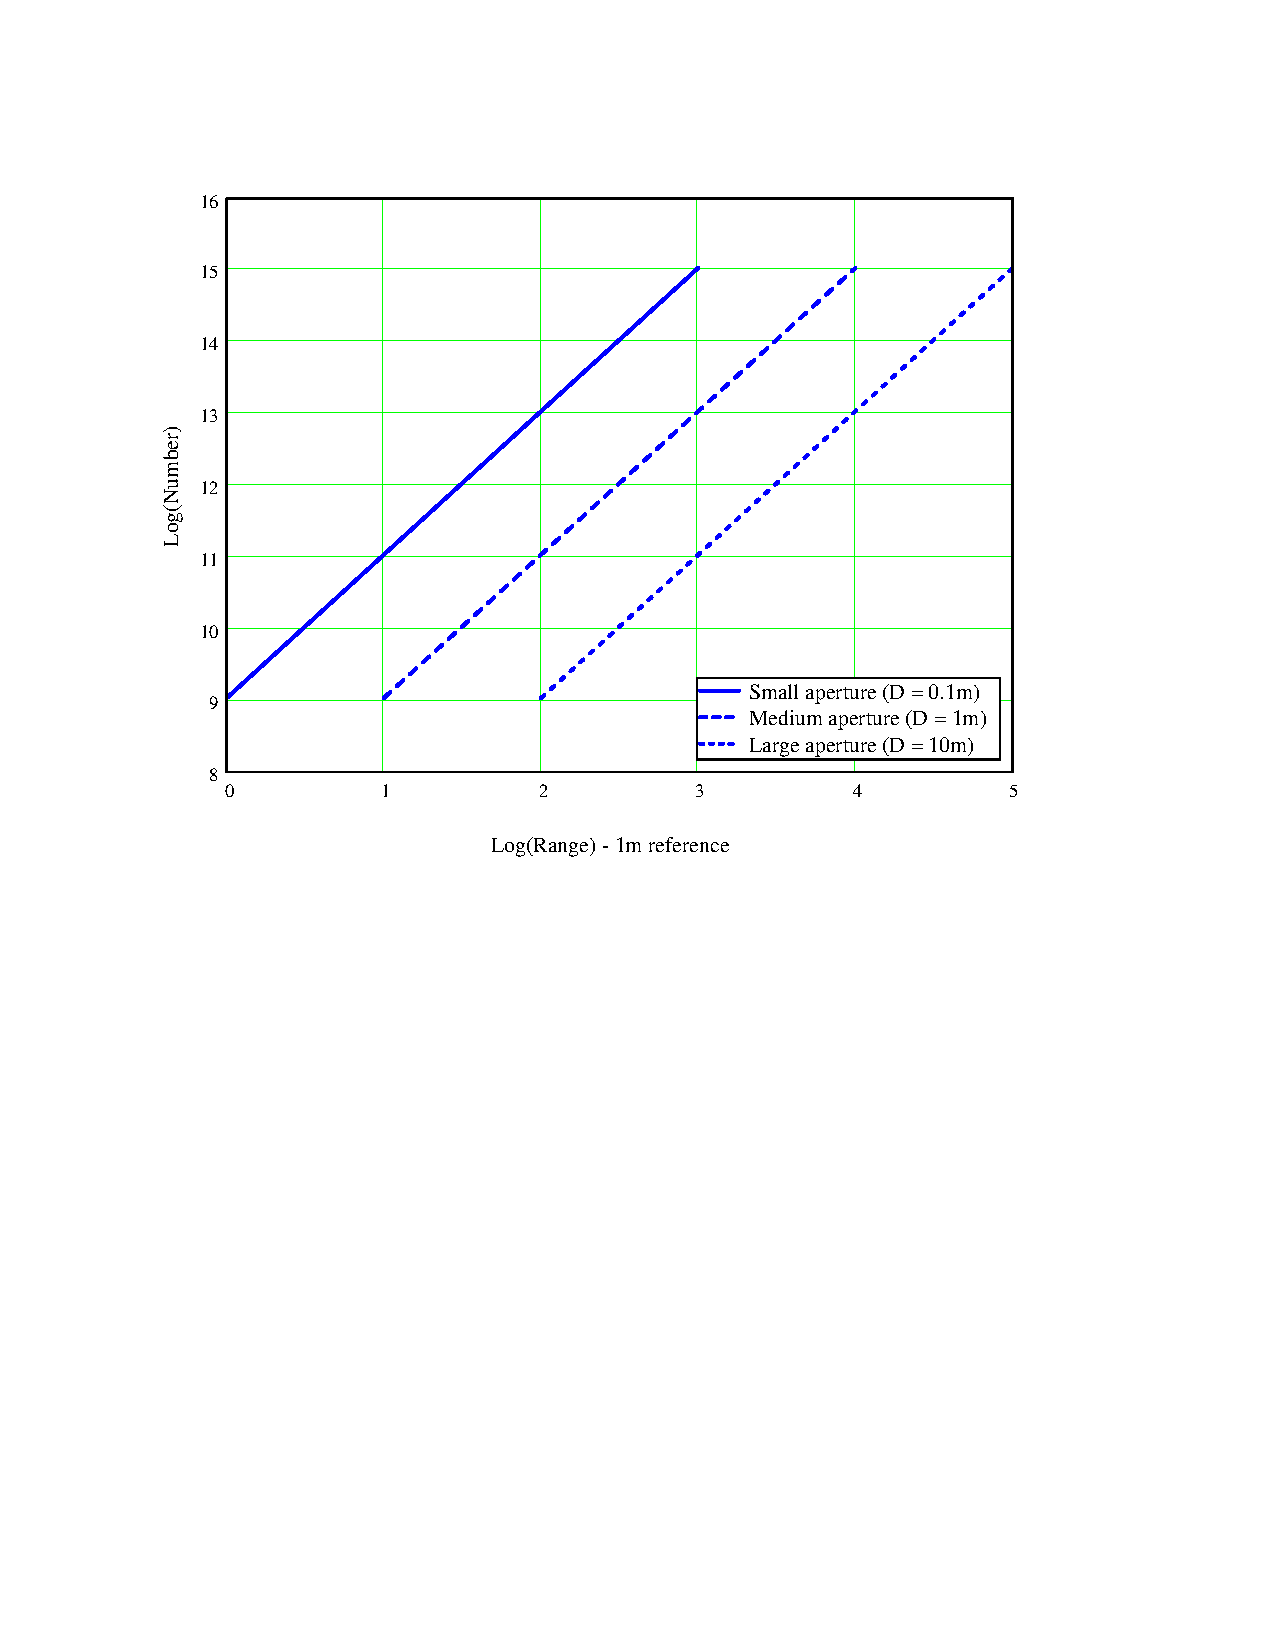
\includegraphics[bb=20 390 489 680]
{back_number/back_number.pdf}
}
\caption[Number of molecules emitting into reciever in a LIDAR application]{Number of molecules emitting into reciever acceptance area (ideal: $A=B=C=D\equiv1$ in Equation \ref{total_prob}). The ratio $R/D$ must be larger than unity to satisfy the approximations used to construct Equations \ref{energy_required} and \ref{v_eff}. Here we have used $\lambda=1$ $\mu$m, and a density of $10^{25}$ molecules per m$^3$. Thus, with an aperture of $D=1$ m and a focal length of 1 km, we expect the system to be sensitive to at most $10^{13}$ atmospheric molecules.}
\label{back_number}
\end{figure}
%----------------------------------------------------------------------------

%----------------------------------------------------------------------------

The output aperture, with diameter $D$, is taken as the origin and the target is at the focus of a Gaussian beam which is some distance, $R$, from the output aperture. The Gaussian beam emerges from the output aperture with a clear aperture compatible with a far-field ripple of less than 1\% \cite{Siegman:1986a}. The integration limits are taken as the boundaries of a rectangular volume centered at the focus: the extent of the region along the beam axis is taken as the Rayleigh range and the transverse dimensions are taken as the waist diameter. The solid angle fraction is taken as
%----------------------------------------------------------------------------
\begin{equation}
\frac{(2\theta)^2}{4\pi}
\end{equation}
%----------------------------------------------------------------------------
where $\theta$ is the far-field divergence \emph{half} angle of the Gaussian beam \cite{Siegman:1986a}. Using these ideas, one can arrive at the following expression for the scaled volume (the product of the volume and the solid angle fraction)
%----------------------------------------------------------------------------
\begin{equation}
\boxed{
V_{eff}
=
\frac{4.6^2}{2 \pi^2}
\lambda^3
\left(\frac{R}{D}\right)^2.
\label{v_eff}
}
\end{equation}
%----------------------------------------------------------------------------
The required pulse energy depends on the fluence (Equation \ref{required fluence}) and the focal spot diameter. The relationship is
%----------------------------------------------------------------------------
\begin{equation}
\boxed{
E
=
\frac{42.32}{\pi}
c \hbar^2 \epsilon_o
\frac{(\Delta\tau)^2}{M^2 t}
\lambda^2
\left(\frac{R}{D}\right)^2.
\label{energy_required}
}
\end{equation}
%----------------------------------------------------------------------------
See Figures \ref{back_number} and \ref{back_energy} for plots of these functions for various aperture sizes.

%----------------------------------------------------------------------------
%----------------------------------------------------------------------------
%bb defines the bounding box for the pdf
%viewport defines the area of the pdf used
%in sidewaysfigure the last entry in bb moves the caption toward/away the pic
%in sidewaysfigure the second entry in bb moves the pic toward/away the caption
%----------------------------------------------------------------------------
\begin{figure}
\scalebox{0.8}[0.8]{
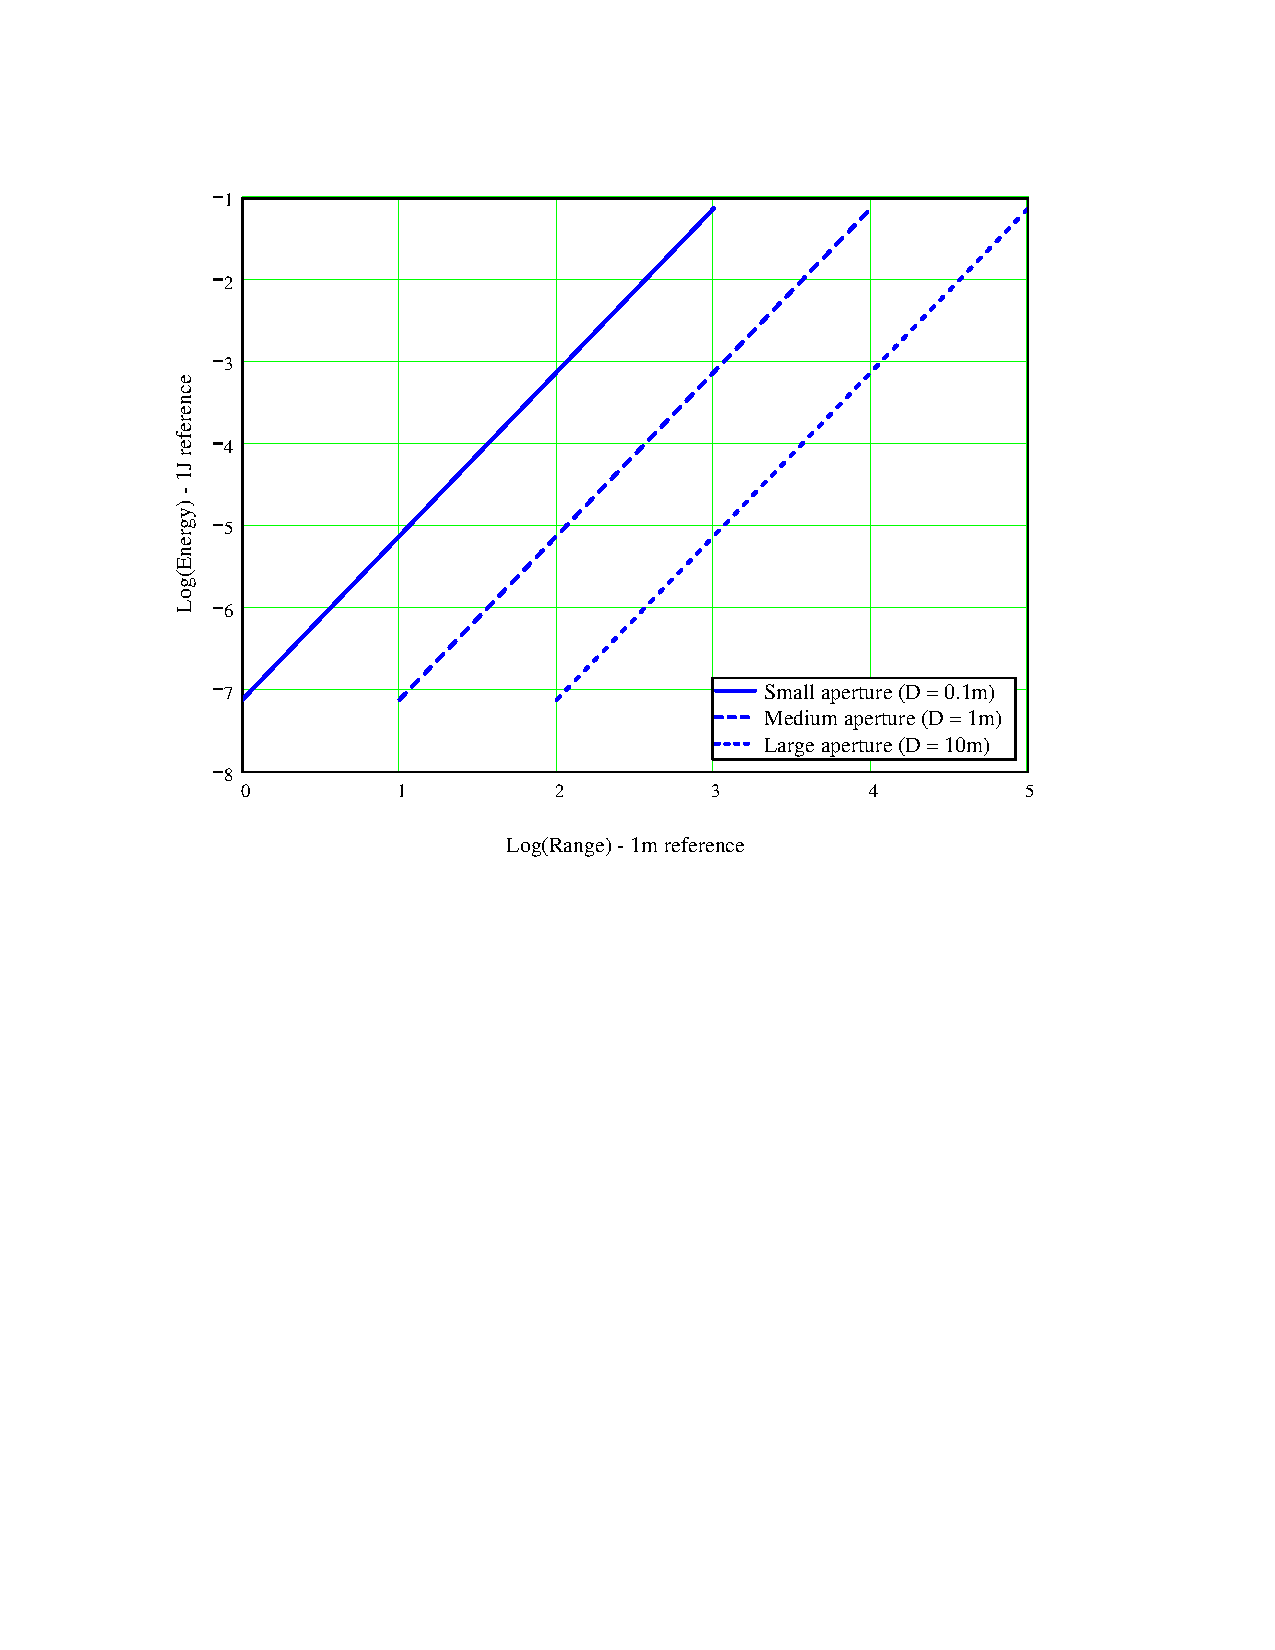
\includegraphics[bb=20 390 489 700]
{back_energy/back_energy.pdf}
}
\caption[Required pulse energy to invert target molecules]{Required pulse energy to invert target molecules. Here we have used the dipole matrix element approximated in Section \ref{iodine} ($M=3.6\cross10^{-32}$ Cm), tophat pulse duration $t=1$ ns, $\lambda=1$ $\mu$m, and $\Delta \tau=\pi/2$ in Equation \ref{energy_required}.}
\label{back_energy}
\end{figure}
%----------------------------------------------------------------------------

%----------------------------------------------------------------------------

The key features of these equations illustrate the potential sensitivity and limitations of LIDAR geometries when one is concerned with LIF type experiments. The effective sensitive volume, Equation \ref{v_eff}, \emph{increases} as the square range, $R$. The obvious drawback is seen in Equation \ref{energy_required} where the required energy also increases with the square of the range. Indeed the ratio
%----------------------------------------------------------------------------
\begin{equation}
\frac{V}{E}
=
\frac{1}{4 \pi c \hbar^2 \epsilon_o}
\frac{M^2 t}{(\Delta\tau)^2}
\lambda
\label{LIDAR eff}
\end{equation}
%----------------------------------------------------------------------------
should be maximized for the most efficient application. $\lambda$ has a natural upper limit set by atmospheric transmission: optical wavelengths greater than 10 um are heavily attenuated. Collisional damping at STP forces $t$ to be less than 1 ns. $\Delta\tau$ is $\pi/2$ for Rabi oscillation population inversion; however, some coherent process require the quantity to increase by an order of magnitude or more (see Chapter \ref{computer chapter}). Most molecules have matrix elements, $M$, around one D ($\mbox{D}=10^{-18}\mbox{ esu}$ and $1\mbox{ Cm}=2.99792458\cross10^{9}\mbox{ esu}$).
%----------------------------------------------------------------------------
%----------------------------------------------------------------------------
